\documentclass{article}
\usepackage[utf8]{inputenc}
\usepackage{verbatim}
\usepackage{mathtools}
\usepackage{float}
\usepackage{graphicx}
\usepackage[]{algorithm2e}
\usepackage{amssymb}
\title{Informe Metodos}
\author{Federico De Rocco}
\date{September 2014}

\usepackage{natbib}
\usepackage{graphicx}

\begin{document}

\maketitle

\section{Introducci\'on}
\section{Matriz Esparsa}
\section{Hits}
\section{PageRank}
\section{In-Deg}
\section{Concluci\'on}
\section{Bibliograf\'ia}

\section{Introducci\'on}
	En este informe se busca explicar tres algoritmos de ranking para p\'aginas de internet. Estos son PageRank, Hits y In-Deg. Dentro de este trabajo se mostrar\'a como se implementaron y se expondr\'an una serie de experimentos para evaluar el funcionamiento de los mismos. 
\section{Matriz Esparsa}
	Por enunciado tenemos que la matriz asociada al grafo posee la caracter\'istica de tener muchos de sus elementos nulos. Se nos da a elegir entre tres posibles implementaciones para esta matriz. Nosotros obtamos por Compressed Sparse Row.
	Esta representaci\'on consta de tres arreglos. El col-ind que es un \'indice de las columnas donde hay un valor distinto de cero. Despu\'es tenemos a row-ptr contiene el \'indice de col-ind de la primera posici\'on de cada fila donde el valor no es nulo. Por ultimo tenemos a vals que contin\'ue todos los valores no cancelados. Este \'ultimo tiene l\'ogicamente el mismo tamaño que col-ind. A modo de ejemplo tenemos la siguiente matriz.

	Las razones de esta elecci\'on son principalmente la ventaja que te provee esta estructura a la hora de multiplicarla por un vector, acci\'on que hacemos muchas veces de forma iterativa, dado que gracias a su forma de guardar y obtener los datos tenemos la oportunidad de hacer menos pasos. Esto se debe a que podemos ignorar las posiciones donde hay ceros. El siguiente es el algoritmo que utilizar\'iamos para obtener el producto de una matriz "normal"(De estructura tipo vector de vectores) con un vector:

\ \\
\begin{algorithm}[H]
\ \\
$n=cantidadDeFilas(Matriz)\in \mathbb{N}$\;
$m=cantidadDeColumnas(Matriz)\in \mathbb{N}$\;
$resultado=(0,0,...,0)\in \mathbb{R}^(n)$\;
 \For{$i=0 ... n-1$}{
  \For{$j=0 ... m-1$}{
 	$resultado_{i}=resultado_{i}+(Matriz_{i,j}*vector_{j})$\;
  }
 }
 $retorna resultado$\;
\caption{Algoritmo de multiplicaci\'on de matriz normal con vector}
\end{algorithm}	
\ \\
Con la matriz esparsa (Compressed Sparse Row) el seudoc\'odigo tendr\'a esta forma:
\ \\
\begin{algorithm}[H]
\ \\
$n=cantidadDeFilas(Matriz)\in \mathbb{N}$\;
$resultado=(0,0,...,0)\in \mathbb{R}^(n)$\;
 \For{$i=0 ... n-1$}{
 	$principioFila=row_ptr_{i}$\;
 	$finalFila=row_ptr_{i+1}$\;
  \For{$j=principioFila ... finalFila-1$}{
 	$resultado_{i}=resultado_{i}+(vector_{col-ind_{j}}*vals_{j})$\;
  }
 }
 $retorna resultado$\;
\caption{Algoritmo de multiplicaci\'on de Compressed Sparse Row}
\end{algorithm}	
\ \\
Como podemos observar en ambos casos debemos ciclar con la cantidad de filas. Pero en el segundo caso tenemos en vez de la cantidad de columnas solo la posici\'on donde se encuentra el primer valor distinto de cero y donde se encuentra el de la siguiente fila. En el caso de que toda la fila sea el vector nulo principioFila y finalFila ser\'an iguales y no se har\'a ninguna cuenta. Dejando a la matriz resultado en ese lugar en 0(Que es el valor que debe tener). Fuera de eso podemos ver que cuando la matriz haga el segundo ciclo, este ser\'a m\'as corto que el del algoritmo de la matriz com\'un. Esto se debe a que al indexar de esta manera nunca pisaremos un valor nulo. Esto \'ultimo es importante porque entre m\'as esparsa sea la matriz mayor ser\'a esta ventaja y menos cuentas adicionales haremos. Adem\'as solo agregamos principioFila y finalFila las cuales solo requieren una asignaci\'on por cada ciclo de i, lo cual no tiene tanto impacto. 
\ \\
La matriz esparsa implementada ten\'ia el problema de la trasposici\'on de la misma. Realizar esta operaci\'on era indispensable para los algoritmos que se deb\'ian hacer us\'andola. Esto era bastante complicado de lograr de una forma eficiente. Por fortuna se llego a la idea de que, en vez de trasponer la matriz, era m\'as conveniente y simple hacer un tipo de multiplicaci\'on especial para traspuesta y vector. Ya que no se necesitaba para otra cosa que para poder usarla en este producto. La funci\'on toma la matriz esparsa y un vector. La idea general se explica en el siguiente seudoc\'odigo:
\ \\
\begin{algorithm}[H]
\ \\
$n=cantidadDeFilas(Matriz)\in \mathbb{N}$\;
$resultado=(0,0,...,0)\in \mathbb{R}^(n)$\;
 \For{$i=0 ... n-1$}{
 	$principioFila=row_ptr_{i}$\;
 	$finalFila=row_ptr_{i+1}$\;
  \For{$j=principioFila ... finalFila-1$}{
 	$resultado_{col-ind_{j}}=resultado_{i}+(vector_{i}*vals_{j})$\;
  }
 }
 $retorna resultado$\;
\caption{Algoritmo de multiplicaci\'on traspuesta de Compressed Sparse Row}
\end{algorithm}	
\ \\
Existe una similitud notable con el de multiplicaci\'on normal expuesto anteriormente en esta secci\'on. Esto se debe a que la \'unica diferencia real es la siguiente linea:
\ \\
$resultado_{col-ind_{j}}=resultado_{i}+(vector_{i}*vals_{j})$\;
\ \\
Puede parecer an\'omalo lo que se propone. Pero la idea general es que fu\'eramos formando el resultado de manera desordenada. Con esto queremos decir que, al terminar el segundo ciclo, no obtengamos el vector con una de su posiciones con el resultado final. En cambio por cada concluci\'on del ciclo habremos cambiado "todas" las posiciones. Esto se traduce en que acumularemos el resultado de una forma diferente para poder obtener lo esperado.

\section{Hits}

Este algoritmo intenta definir una noci\'on de autoridad utilizando los links que apuntan a una determinada p\'agina. Se considera que hay algunas de estas que cumplen un rol de autoridad sobre un tema espec\'ifico y se busca una relaci\'on entre estas y las p\'aginas que apuntan a varias autoridades, estas \'ultimas se denominan hubs. Consideramos que un hub bueno es el que apunta a muchas autoridades buenas y que una autoridad buena lo es cuando es apuntada por muchos hubs buenos. Se nos da una sub-red y se nos dice que consideremos que las p\'aginas asociadas a esta se encuentran en $Web=(0,...,n)$. Tomamos la matriz de adyacencia $A{0,1}\in \mathbb{R}^(n*n)$ , en esta matriz tenemos que $a_{i,j}=1$ si y solo si existe un link de la p\'agina i a la j. Para todas las p\'aginas se considera $x_{i}$ como el peso de autoridad y $y_{i}$ el peso de los hubs. Los vectores de pesos de autoridad y de hubs son x \'e y respectivamente, con $x, y \in \mathbb{R}^(n)$.  
En resumen, podemos decir que:
\ \\
\[
x_{j}=\sum_{i:i->j}y_{i} 
\]
\[
y_{i}=\sum_{j:i->j}x_{j} 
\]
\ \\
Esta es la expreci\'on num\'erica de lo anterior mostrado. Como estamos trabajando con matrices podemos ver que estas formulas son equivalentes a:
\ \\
$x=\mathbb{A}^(t)*y$
\ \\
$y=A*x$
\ \\
Hay que recordad que se deben aplicar los pasos de normalizaci\'on para ambos vectores una vez terminados estos productos. Como sugiere el autor Jon M. Kleinberg, comenzaremos usando un vector inicial el cual tendr\'a el tamaño adecuado para realizar la operaci\'on anterior y que adem\'as tenga en todos sus valores unos. Seg\'un el paper esto, bajo ciertas condiciones, converger\'ia hasta darnos una noci\'on m\'as acertada de los pesos de autoridades y hubs. Para poder realizar el algoritmo propuesto se considera el siguiente seudoc\'odigo:
\ \\
\begin{algorithm}[H]
\ \\
$k\in \mathbb{N}$\;
$x=(1,1,...,1)\in \mathbb{R}^(n)$\;
 \For{$i=0 ... n-1$}{
 	$x=Matriz*y$\;
 	$y=Matriz*x$\;
 	$x=normalizar(x)$\;
 	$y=normalizar(y)$\;
}
 $retorna$ $tupla_{x,y}$\;
\caption{Algoritmo Iterativo de Hits}
\end{algorithm}	
\ \\


\section{Creaci\'on}
\ \\
El objetivo de este algoritmo es crear la \textit{matriz de conectividad W} $\in$ $\mathbb{R}^{n\times n}$, siendo \textit{n} la cantidad de p\'aginas web de las que deberemos evaluar su importancia a trav\'es de distintos algoritmos, de forma tal que $w_{ij}$=1 si la p\'agina \textit{j} tiene un link a la p\'agina \textit{i} y $w_{ij}$=0 en caso contrario. Tambi\'en hay que tener en cuenta de que los \textit{autolinks} son ignorados, es decir que $w_{ii}$=0. Esta se crear\'a a partir del grafo que representa la red de p\'aginas, cuya particularidad es que posee muchos 0's puesto que posee pocos links de salida en comparaci\'on con el n\'umero total de p\'aginas. Cuando \textit{n} es un n\'umero muy grande, debemos elegir una estructura de representaci\'on adecuada para no perder memoria y solo guardar los datos que nos interesan. Por esta raz\'on es que la matriz \textit{W} se representa con una matriz esparza. Hemos elegido utilizar la representaci\'on a trav\'es de la \textit{Compressed Sparse Row}. Una de las principales razones de nuestra selecci\'on fue debido a la ventaja que te provee esta estructura a la hora de multiplicarla por un vector (que es la \'unica operaci\'on que realizaremos sobre esta), acci\'on que haremos muchas veces de forma iterativa. Esto se debe a que podemos ignorar las posiciones donde hay ceros y, como nuestra matriz los posee en gran cantidad, este algoritmo se realizar\'a m\'as r\'apido que si estuvi\'esemos trabajando con una matriz tradicional junto con su respectiva multiplicaci\'on. La manera de representar esta matriz es a trav\'es de 3 vectores. Uno de ellos es el que hemos llamado \textit{col ind}, el cual indicar\'a los \'indices de las columnas donde hay un valor distinto de cero en la matriz de manera ordenada, es decir que ir\'a recorriendo de a filas y colocando estos valores, indexando desde 0. Un ejemplo puede ser este: Supongamos que tenemos una matriz cuya primer fila est\'a dada por el vector $[$0 0 1 1$]$, luego los primeros valores de este vector \textit{col ind} ser\'an $[$2 3$]$ debido a que en la columna 2 y 3 hay valores distintos de 0. Otro de los vectores que poseemos en la estructura es llamado \textit{row ptr}, el cual contiene el \'indice de \textit{col ind} de la primera posici\'on de cada fila donde el valor no es nulo. Para ser m\'as claros, mostremos un ejemplo: Consideremos el vector tomado en el ejemplo anterior y tomemos una segunda fila de la matriz dada por el vector $[$1 0 0 0$]$. Ahora nuestros primeros valores de \textit{col ind} ser\'an $[$2 3 0$]$ y, entonces, los valores de \textit{row ptr} que tenemos hasta ahora ser\'an $[$0 2$]$, indicando que el elemento en la posici\'on 0 de \textit{col ind} es el primer valor distinto de 0 de la primer fila de la matriz original y que el elemento de la posici\'on 2 es el primero distinto de 0 de la siguiente fila. Cuando nos encontramos en el caso en el que una fila posee todos 0's, luego en \textit{row ptr} se repetir\'a el \'ultimo valor tomado. Por ejemplo, si la segunda fila de la matriz tomada anteriormente hubiese tenido todos 0's y tuvi\'esemos ahora una tercer fila cuyos valores fuesen los $[$1 1 0 1$]$, ahora tendr\'iamos un \textit{col ind}=$[$2 3 0 1 3$]$, y entonces los valores hasta ahora que poseemos en \textit{row ptr} ser\'ian $[$0 2 2$]$ indicando que en la primer fila hab\'ian dos valores y luego en la segunda no hab\'ia ninguno, por eso es que el 2 se repite. El \'ultimo vector que poseemos es el llamado \textit{vals} que contiene el valor correspondiente en la matriz de cada elemento en correspondencia con el \textit{col ind}, es decir que si tomamos el \'ultimo ejemplo tomado y consideramos que el primer valor distinto de 0 en la primer fila era el 3, luego en la primer posici\'on de \textit{vals} tendremos un 3. Es claro ver que este vector debe poseer el mismo tamaño que \textit{col ind} puesto que le corresponde a cada elemento de este \'ultimo su valor. Una vez realizado esto, ya tenemos nuestra matriz esparza (la cual sufrir\'a una pequeña modificaci\'on de la que se hablar\'a en el siguiente p\'arrafo). Posteriormente se mostrar\'a una secci\'on en la que se hablar\'a de las operaciones de multiplicaci\'on de esta matriz ya que se realizan de manera especial debido a su representaci\'on y puesto que es la \'unica operaci\'on que realizaremos con ella. 
\ \\
Continuando con la explicaci\'on de la creaci\'on de la matriz, ahora se hablar\'a del algoritmo habiendo ya explicado el tipo de representaci\'on que utilizaremos y c\'omo est\'a formada la matriz. Para este algoritmo trabajaremos con los vectores \textit{x} e \textit{y}, cuyas posiciones formar\'an una tupla \textit{i,j} que indican que \textit{i} est\'a apuntando a la p\'agina \textit{j}, es decir que si x$[0]=$1 e y$[$0$]$=3, luego esto formar\'a la tupla $[1$ $3]$ en la cual la p\'agina 1 est\'a apuntando a la 3. Crearemos un nuevo vector llamado \textit{resParciales} que contendr\'a \textit{n} vectores de ints, cada uno conteniendo todas las p\'aginas que sigan a aquella que corresponde al valor de la posici\'on del vector m\'as 1. Esto quiere decir que en la posici\'on 0 del vector se encontrar\'an todas aquellas p\'aginas que siguen a la 1. El siguiente paso es realizar un algoritmo de sorting sobre cada uno de estos vectores generados, en particular hemos utilizado uno prove\'ido por una librer\'ia de c++. La raz\'on por la que realizamos esto es porque en cada fila de la matriz \textit{W} tendremos un 1 en aquella columna cuya posici\'on indica que esta p\'agina sigue a la 1, luego si tenemos todos estos valores y ordenados de manera creciente, solo basta colocarlos en \textit{col ind} para crear la matriz deseada, siempre recordando que como indexamos desde 0 luego si tenemos un 2 en \textit{col ind} esto significa que en verdad es la p\'agina 3 de la que hablamos. Para pasar los valores a \textit{col ind}, primero nos fijamos si esa fila es nula, en la cual deberemos solamente colocar en \textit{row ptr} el \'ultimo valor que fue agregado. En el caso contrario, procedemos a agregar en \textit{col ind} los valores correspondientes a la iteraci\'on que estamos realizados del vector de vectores \textit{resParciales} (rest\'andole 1 pues indexamos desde 0 la matriz), esto quiere decir que si estamos en la iteraci\'on 0 del ciclo, colocaremos todos los valores del vector 0 de \textit{resParciales}. Luego agregaremos un 1 a \textit{vals} puesto que esta matriz solo tiene 0's y 1's y, finalmente, agregaremos a \textit{row ptr} un valor que ser\'a la suma del valor anteriormente ingresado a este vector con la cantidad de valores no nulos de la fila correspondiente a la iteraci\'on anterior que realizamos (si estamos en la primer fila entonces se agregar\'a un 0), es decir que si antes agregamos 2 valores y ten\'iamos un 0 en \textit{row ptr}, ahora deberemos agregar un 2. Luego de realizar todos los ciclos, se proceder\'a a agregar una \'ultima operaci\'on, la cual agregar\'a a \textit{row ptr}  el tamaño de \textit{col ind}. Esto se realiza debido a que facilita el algoritmo de multiplicaci\'on de este tipo de matriz, la cual ser\'a explicada en la pr\'oxima secci\'on. Teniendo en cuenta esta diferencia respecto a lo explicado antes sobre como estaba representada la matriz esparza, si alguien desease reconstruir una matriz a partir de nuestra esparza, deber\'ia tener en cuenta este hecho a la hora de hacerlo para ignorar el \'ultimo valor agregado en \textit{row ptr}.
\ \\
A continuaci\'on presentaremos un pseudoc\'odigo que muestra lo hablado anteriormente:
\ \\
\begin{algorithm}[H]
Crear vector \textit{resParciales} de tamaño n\\
\For{Cada elemento i menor al tamaño del vector x, y}{
	 Agregar a la posi\'on (y$[$i-1$]$) de \textit{resParciales} el valor que se encuentra en (X$[i]$)
}	
\For{Cada subvector de \textit{resParciales}}{
	 ordenar\
	 int cantValores = 0\
}
\For{Cada subvector de \textit{resParciales}}{
	\eIf{Subvector es de tamaño nulo}{
		 Agregar a row ptr cantValores\
		 }{
		\For{Cada elemento del subvector elegido}{
			 Agregarlo a col ind\
			 Agregar a vals 1\
		}
		 Agregar a row ptr cantValores\
		 Sumar a cantValores la cantidad de elementos del subvector\
	}			
}
Agregar a row ptr un valor que es el tamaño de col in\
\caption{Algoritmo de creaci\'on de matriz W}
\end{algorithm}
\ \\
\subsection{Multiplicando matrices esparzas}
Ya hemos hablado anteriormente sobre qu\'e son las matrices esparzas. Para refrescar su memoria, \'estas son matrices cuya particularidad es que posee muchos elementos nulos en comparaci\'on con aquellos que no lo son. Por esta raz\'on es que se utiliza un particular modo de representaci\'on de la matriz para as\'i ocupar menos espacio, guardando solamente los datos de los valores no nulos. Sobre esta matriz y su transpuesta solo realizaremos multiplicaciones con vectores (puesto que esto nos basta para realizar los algoritmos que deseamos). Para realizar esta \'ultima, necesitamos realizar algunas modificaciones a las multiplicaciones cl\'asicas de matrices con vectores debido a su particular representaci\'on. Este algoritmo toma una Matriz que llamaremos Matriz y un vector que llamaremos vector para realizarse. A continuaci\'on mostraremos un pseudoc\'odigo sobre la implemetanci\'on de esta misma, seguido de una breve explicaci\'on:
\ \\
\begin{algorithm}[H]
\ \\
$n=cantidadDeFilas(Matriz)\in \mathbb{N}$\\
$resultado=(0,0,...,0)\in \mathbb{R}^(n)$\\
 \For{$i=0 ... n-1$}{
 	$principioFila=row_ptr_{i}$\;
 	$finalFila=row_ptr_{i+1}$\;
  \For{$j=principioFila ... finalFila-1$}{
 	$resultado_{i}=resultado_{i}+(vector_{col-ind_{j}}*vals_{j})$\;
  }
 }
 $retorna$ $resultado$\;
\caption{Algoritmo de multiplicaci\'on de Compressed Sparse Row}
\end{algorithm}	
\ \\
Como cuando multiplicamos una matriz cl\'asica contra un vector, ciclaremos sobre las filas. La diferencia de esta forma de multiplicar es que tenemos solo la posici\'on donde se encuentra el primer valor distinto de cero y donde se encuentra el de la siguiente fila, en vez de poseer una fila entera. En el caso de que toda la fila sea el vector nulo, \textit{principioFila} y \textit{finalFila} ser\'an iguales y no se har\'a ninguna cuenta, dejando al vector resultado como estaba antes. Cuando nos encontremos en el caso contrario, la matriz pasar\'a a realizar el segundo ciclo, el cual ser\'a m\'as r\'apido que el del algoritmo de la matriz c\'asico debido a que al tener este tipo de representaci\'on, nunca realizaremos operaciones sobre filas vac\'ias o sobre valores nulos, ahorr\'andonos ese tiempo perdido. Esto \'ultimo es importante porque entre m\'as esparza sea la matriz, mayor ser\'a esta ventaja y menos cuentas adicionales haremos. Luego lo que haremos en ese segundo ciclo ser\'a multiplicar con el vector los valores no nulos de la fila correspondiente de la matriz, es decir aquellos que tenemos guardados en la representaci\'on puesto que el resto de los valores ser\'ian multiplicados por 0 y esto no influir\'ia sobre el resultado. Esta multiplicaci\'on ser\'a como la cl\'asica de las matrices, solo que tomar\'a en cuenta los \'indices del vector que no vayan a ser multiplicados por 0 (es decir, aquellas posiciones que est\'an definidas en \textit{col ind}. Una vez realizado todo esto sobre cada fila, ya tenemos nuestro vector resultado.
\ \\
Para los algoritmos con los que trabajaremos necesitamos utilizar la matriz transpuesta de la esparza, lo cual es dif\'icil de conseguir debido a la representaci\'on de la misma. Pudimos llegar a la conclusi\'on de que, en vez de transponer la matriz, era m\'as conveniente y simple hacer un tipo de multiplicaci\'on especial para la transpuesta con un vector, ya que no se necesitaba m\'as que para realizar esta operaci\'on. La idea general se explica en el siguiente pseudoc\'odigo, seguido de una breve explicaci\'on del mismo:
\ \\
\begin{algorithm}[H]
\ \\
$n=cantidadDeFilas(Matriz)\in \mathbb{N}$\\
$resultado=(0,0,...,0)\in \mathbb{R}^(n)$\\
 \For{$i=0 ... n-1$}{
 	$principioFila=row_ptr_{i}$\;
 	$finalFila=row_ptr_{i+1}$\;
  \For{$j=principioFila ... finalFila-1$}{
 	$resultado_{col-ind_{j}}=resultado_{i}+(vector_{i}*vals_{j})$\;
  }
 }
 $retorna$ $resultado$\;
\caption{Algoritmo de multiplicaci\'on transpuesta de Compressed Sparse Row}
\end{algorithm}	
\ \\
Existe una similitud notable con el de multiplicaci\'on expuesto anteriormente en esta secci\'on. Esto se debe a que la \'unica diferencia real es la siguiente linea:
\ \\
\begin{center}
$resultado_{col-ind_{j}}=resultado_{i}+(vector_{i}*vals_{j})$\;
\end{center}
\ \\
Puede parecer an\'omalo lo que se propone, pero la idea general es que fu\'eramos formando el resultado de manera desordenada. Con esto queremos decir que, al terminar el segundo ciclo, no obtengamos el vector con una de su posiciones con el resultado final. En cambio por cada conclusi\'on del ciclo habremos cambiado todas las posiciones. Esto se traduce en que acumularemos el resultado de una forma diferente para poder obtener lo esperado. De esta forma pudimos obtener un vector cuyo resultado es la multiplicaci\'on de una matriz esparza transpuesta por un vector.

\section{PageRank}
\section{In-Deg}
\section{Experimentos}
\section{Experimentos de convergencia}
Para estas pruebas utilizando los algoritmos de Hits y PageRank utilizaremos las siguientes instancias de experimentaci\'on.
\ \\
Primera instancia: CA-GrQc, Sacada de [4].
\ \\
Segunda instancia: CA-HepTh, Sacada de [5].
\ \\
\section{Estudio de Convergencia de Hits}

Tomaremos las dos instancias de tamaño medio-grande y observaremos que tan r\'pido converge variando la cantidad de iteraciones del algoritmo. Para esto calcularemos los hubs y autoridades usando un k entre 1 y 10. Si el m\'etodo converge, la diferencia entre los resultados y el de la muestra con k=10 ser\'ia cada vez menor. La diferencia entre dos vector es la resta de cada elemento del vector en m\'odulo, este resultado es tambi\'en un vector. Si hacemos la sumatoria de el vector de diferencias, veremos que cada vez es m\'as cercana a el valor nulo. Con esto podemos ver que la diferencia entre cada valor del vector se va acercando a 0. Sean $x, y , vectorDiferencias\in \mathbb{R}^(n)$. La diferencia entre x e y se representa de la siguiente forma: 
\ \\

$vectorDiferencias_{i}=abs(x_{i}-y_{i})$ $\forall i<tamaño(x) \in \mathbb{N}$  

\ \\
Por otro lado la sumatoria de un vector se representa de la siguiente manera:
\ \\
\[
resultado=resultado+\sum_{i=1:i->n}vectorDiferencias_{i} 
\]
\ \\
Con $resultado \in \mathbb{R}$ tal que al iniciar la sumatoria $resultado=0$. Esto nos muestra que el m\'etodo converge. Para medir esto calculamos con los k mencionados. Y vimos la sumatoria de las diferencias entre k=10 y cada uno de los dem\'as. Tambi\'en descartamos el resultado en el caso k=1 ya que las diferencias eran muy grande por solo iterar una vez y no nos permit\'ia apreciar el gr\'afico. Las siguientes im\'agenes muestran el resultado. 
\ \\
\begin{figure}[H]
  \centering
    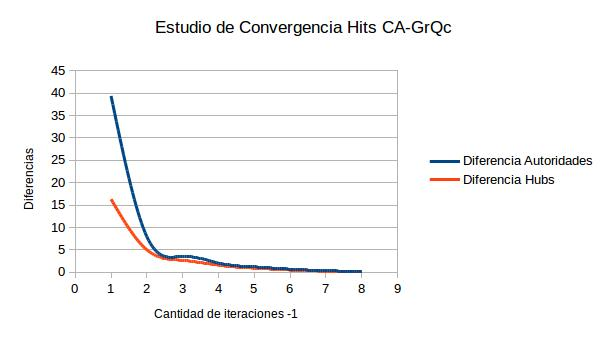
\includegraphics[width=0.7\textwidth]{ConvergenciaHits}
\end{figure}
\ \\
\ \\
\begin{figure}[H]
  \centering
    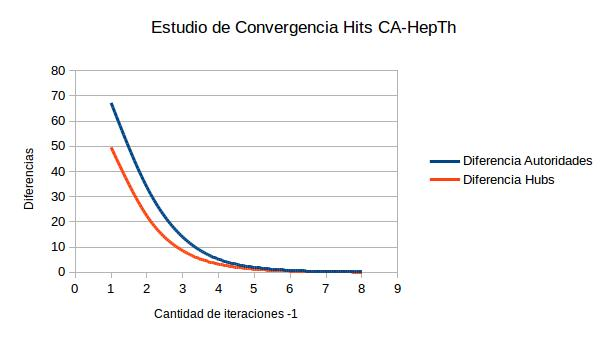
\includegraphics[width=0.7\textwidth]{ConvergenciaHits2}
\end{figure}
\ \\

El primero es usando la muestra CA-GrQc y el segundo es con CA-HepTh. Como podemos ver el gr\'afico nos muestra que entre m\'as cerca estemos del k=10 la suma de las diferencias, tanto de hubs como de autoridades, se acerca a 0. Esto nos dice que las diferencias son siempre menores. Por lo tanto el m\'etodo converge.

\section{Experimentos de Tiempos}
En esta parte observaremos los tiempos para los dos algoritmos. Para lograr esto usaremos una herramienta de C++, incluida en la librer\'ia time.h, nombrada como la funci\'on clock(). Devuelve el tiempo de procesador consumido por el programa. El valor devuelto se expresa en ciclos de reloj, que son unidades de tiempo de una longitud constante, pero espec\'ifico del sistema (con una relaci\'on de CLOCKS-PER-SEC tics del reloj por segundo). Con este tomaremos el tiempo al iniciar el programa, justo antes de cargar variables, y lo volveremos a tomar cuando este termine. Restando ambos valores y dividi\'endolo por la constante nombrada anteriormente conseguiremos el tiempo en segundos que se tardo nuestro algoritmo.

Tomando las muestras del experimento de convergencia, realizaremos mediciones variando la cantidad de iteraciones. Usamos Hits variando el k(cantidad de iteraciones) de 11, 14, 17, 20, 23, 26, 29, 32, 35, 38, 41. Esto \'ultimo se debe a que ambos alcanzan el resultado en k=11. Fuimos saltando de a 3 para que se viera mejor en el gr\'afico.Tomamos 10 tiempos distintos para cada k y sacamos los dos m\'aximos y los dos m\'inimos para no considerar los casos bordes. Luego calculamos el promedio.  

Para CA-GrQc y CA-HepTh en Hits nos dio:
\ \\
\begin{figure}[H]
  \centering
    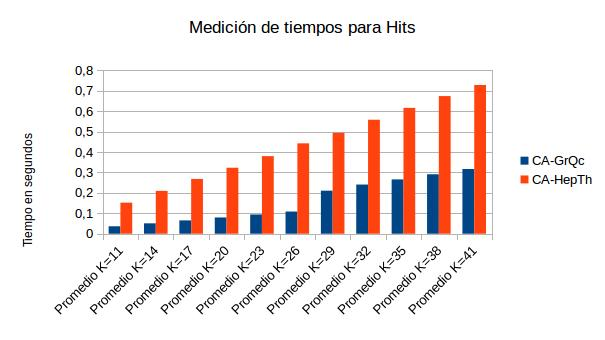
\includegraphics[width=0.7\textwidth]{tiemposHits1}
\end{figure}
\ \\
Con esto podemos tener una idea de como aumenta el tiempo que tarda el algoritmo dependiendo de la cantidad de iteraciones. Esto es importante porque nos muestra que tanto impacta en tiempo de c\'omputo si ponemos un k innecesariamente grande.

\section{Concluci\'on}
\section{Bibliograf\'ia}

\begin{thebibliography}{5}

\bibitem{kleinberg}
  Kleinberg,
  \emph{Authoritative sources in a hyperlinked environment secciones 1, 2 y 3}.
  1999.
\bibitem{bryanLeise}
  Bryan, Leise,
  \emph{The Linear Algebra behind Google}.
  2006.
\bibitem{kamvar}
  Kamvar, Haveliwala,
  \emph{Extrapolation methods for accelerating PageRank computations}.
  2003.
  \bibitem{kamvar}
  P\'agina de internet,
  \emph{http://snap.stanford.edu/data/CA-GrQc.html}.
    \bibitem{kamvar}
  P\'agina de internet,
  \emph{http://snap.stanford.edu/data/CA-HepTh.html}.

\end{thebibliography}

\end{document}